The Cryogenic Underground Observatory for Rare Events (CUORE) \cite{Ardito:2005ar}
has been designed following the successful experience of the  MiDBD \cite{Arnaboldi:2002te} and Cuoricino \cite{Andreotti:2010vj} $^{130}$Te experiments, where for the first time arrays of bolometers were used to search for $\beta\beta$ decay.

CUORE will be placed in the hall A of the Gran Sasso Underground Laboratory and will consist of a system of 988 bolometers, each being a crystal of TeO$_2$ of $5\times5\times5$ cm$^3$, arranged in 19 vertical towers consisting of 13 layers of 4 crystals each. The four crystals are held between two copper frames joined by copper columns. PTFE pieces are inserted between the copper and TeO$_2$, as a heat impedance and to clamp the crystals. There is a few mm gap between crystals with no material between them.
A system of lead shields will be hosted inside the cryostat close to the detectors, to shield them from environmental radioactivity and from radioactive contaminations originating in the dilution unit located above the detector and in the dewar structure \cite{Bellini:2007zz}. A 6 cm thick roman lead shield surrounds the detector array on its sides, while a 30 cm thick layer of low-activity lead is placed above the detector. The $^{210}$Pb activity of the roman lead was measured to be less than 4 mBq/kg. A sketch of the detector is shown in fig.~\ref{fig:cuore}.

%%%%%
\begin{figure}[t!]
\begin{center}
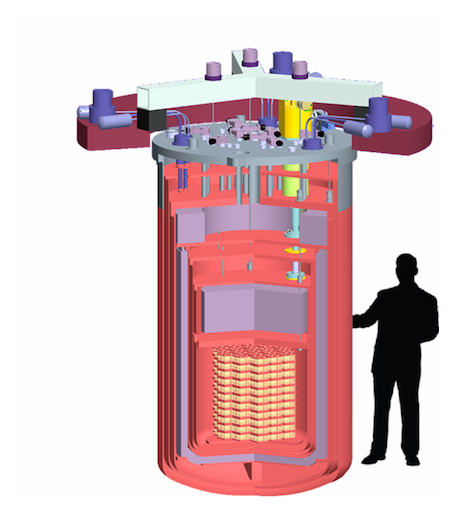
\includegraphics[scale=.8]{img/cuore.eps}
\end{center}
\caption{The CUORE detector and cryostat. In yellow, the 19 towers of bolometers; the lavender volumes are the lead shielding.}\label{fig:cuore}
\end{figure}
%%%%%

The total mass of the detector will be 741 kg for a $^{130}$Te mass of 206 kg. The energy released in a single particle interaction within the crystal is measurable as a change in temperature by  Neutron Transmutation Doped (NTD) germanium thermistors. The measured energy resolution is $\sim 5$ keV FWHM at the $\beta \beta \; (0\nu)$ transition energy ($\sim 2.53$ MeV).

The CUORE bolometers will operate at temperatures between 10 and 15 mK. A challenging $^3$He/$^4$He dilution refrigerator, with a cooling power of 3 mW at 120 mK, has been designed on purpose and is under construction.

A single tower of CUORE, CUORE-0, is presently under construction and will begin  operations within 2011. It will be hosted in the old Cuoricino dilution refrigerator, placed in the hall A of the LNGS. CUORE-0 is a real test of the CUORE assembly chain and procedure, will directly test the level of backgrounds of the CUORE setup and improve the Cuoricino sensitivity on \bbonu.

The CUORE setup will possibly allow in the long term for powerful upgrades. An obvious, though expensive, possibility is to substitute the natural tellurium bolometers with enriched $^{130}$Te units (provided that the enrichment procedure can keep the internal backgrounds very low). A more sophisticated option is to use scintillating crystals containing interesting double beta emitters \cite{Pirro:2005ar}. The contemporary read-out of scintillation light and thermal signal could indeed allow for a dramatic reduction of the background rate and a better characterization of the signal. An array of ZnSe scintillating bolometers, LUCIFER, has been recently proposed as a prototype experiment exploring the performances of such an approach \cite{Ferroni:2011zz} (see sect.~\ref{subsec:other}).


